% !TEX TS-program = xelatex
% !TEX encoding = UTF-8 Unicode

\providecommand{\home}{../..}
\documentclass[\home/main.tex]{subfiles}

\begin{document}

\chapter{Citizen science for robotic folding}\label{ch:data_collection}

%  Problem statement + why traditional and SOTA methods cannot solve it
Deep reinforcement learning is being applied to many robotic manipulation problems such as grasping everyday objects \autocite{Levine2018},~peg-hole insertion \autocite{Finn2016}, and bin-picking tasks \autocite{Mahler2019}. However, applications concerning the manipulation of deformable objects are scarce due to their highly complex behavior caused by deformations \autocite{Foresti2004}. Clothing, in particular, is a problem relevant to household robotics and industry. While existing work engineers highly complex pipelines \autocite{Doumanoglou2016, Maitin2010} with predefined end-effector trajectories \autocite{Miller2012}, some authors recently tried tackling the problem by learning the required manipulation skills \autocite{Matas2018, Seita2018}. These methods require many demonstrations and are trained in simulation, which can lead to transferability issues. Additionally, defining a reward function for the robotic folding problem is hard because of the high dimensionality of the state of textile objects. \par 

% Waarom menselijke taak voorbeelden nuttig zijn maar de huidige datasets voor robot folding task niet genoeg zijn
Prior work has shown that it is possible to bootstrap learning by starting from task demonstrations \autocite{Vevcerik2017} or learn the reward function from expert samples \autocite{Abbeel2004}. Learning skills from human demonstrations also provides a communication medium from human to robot, enabling non-experts to train robots or learn from video websites. Datasets containing task executions are useful in this regard as they help research in learning from human demonstrations. For example, the MIME dataset \autocite{Sharma2018} consists of video demonstrations of 20 different tasks. However, only one task deals with deformable objects, the video stream is single-view RGB-D data, and the task consists of wiping with a cloth which is considerably less complicated compared to folding clothing. Datasets that deal exclusively with clothing, for example, DeepFashion \autocite{Liu2016} mainly focuses on cloth recognition tasks making them hard to use for learning the robotic folding task.

%TODO: op de figuur de onderdelen aanduiden? 
\begin{figure}[htpb]
    \centering
    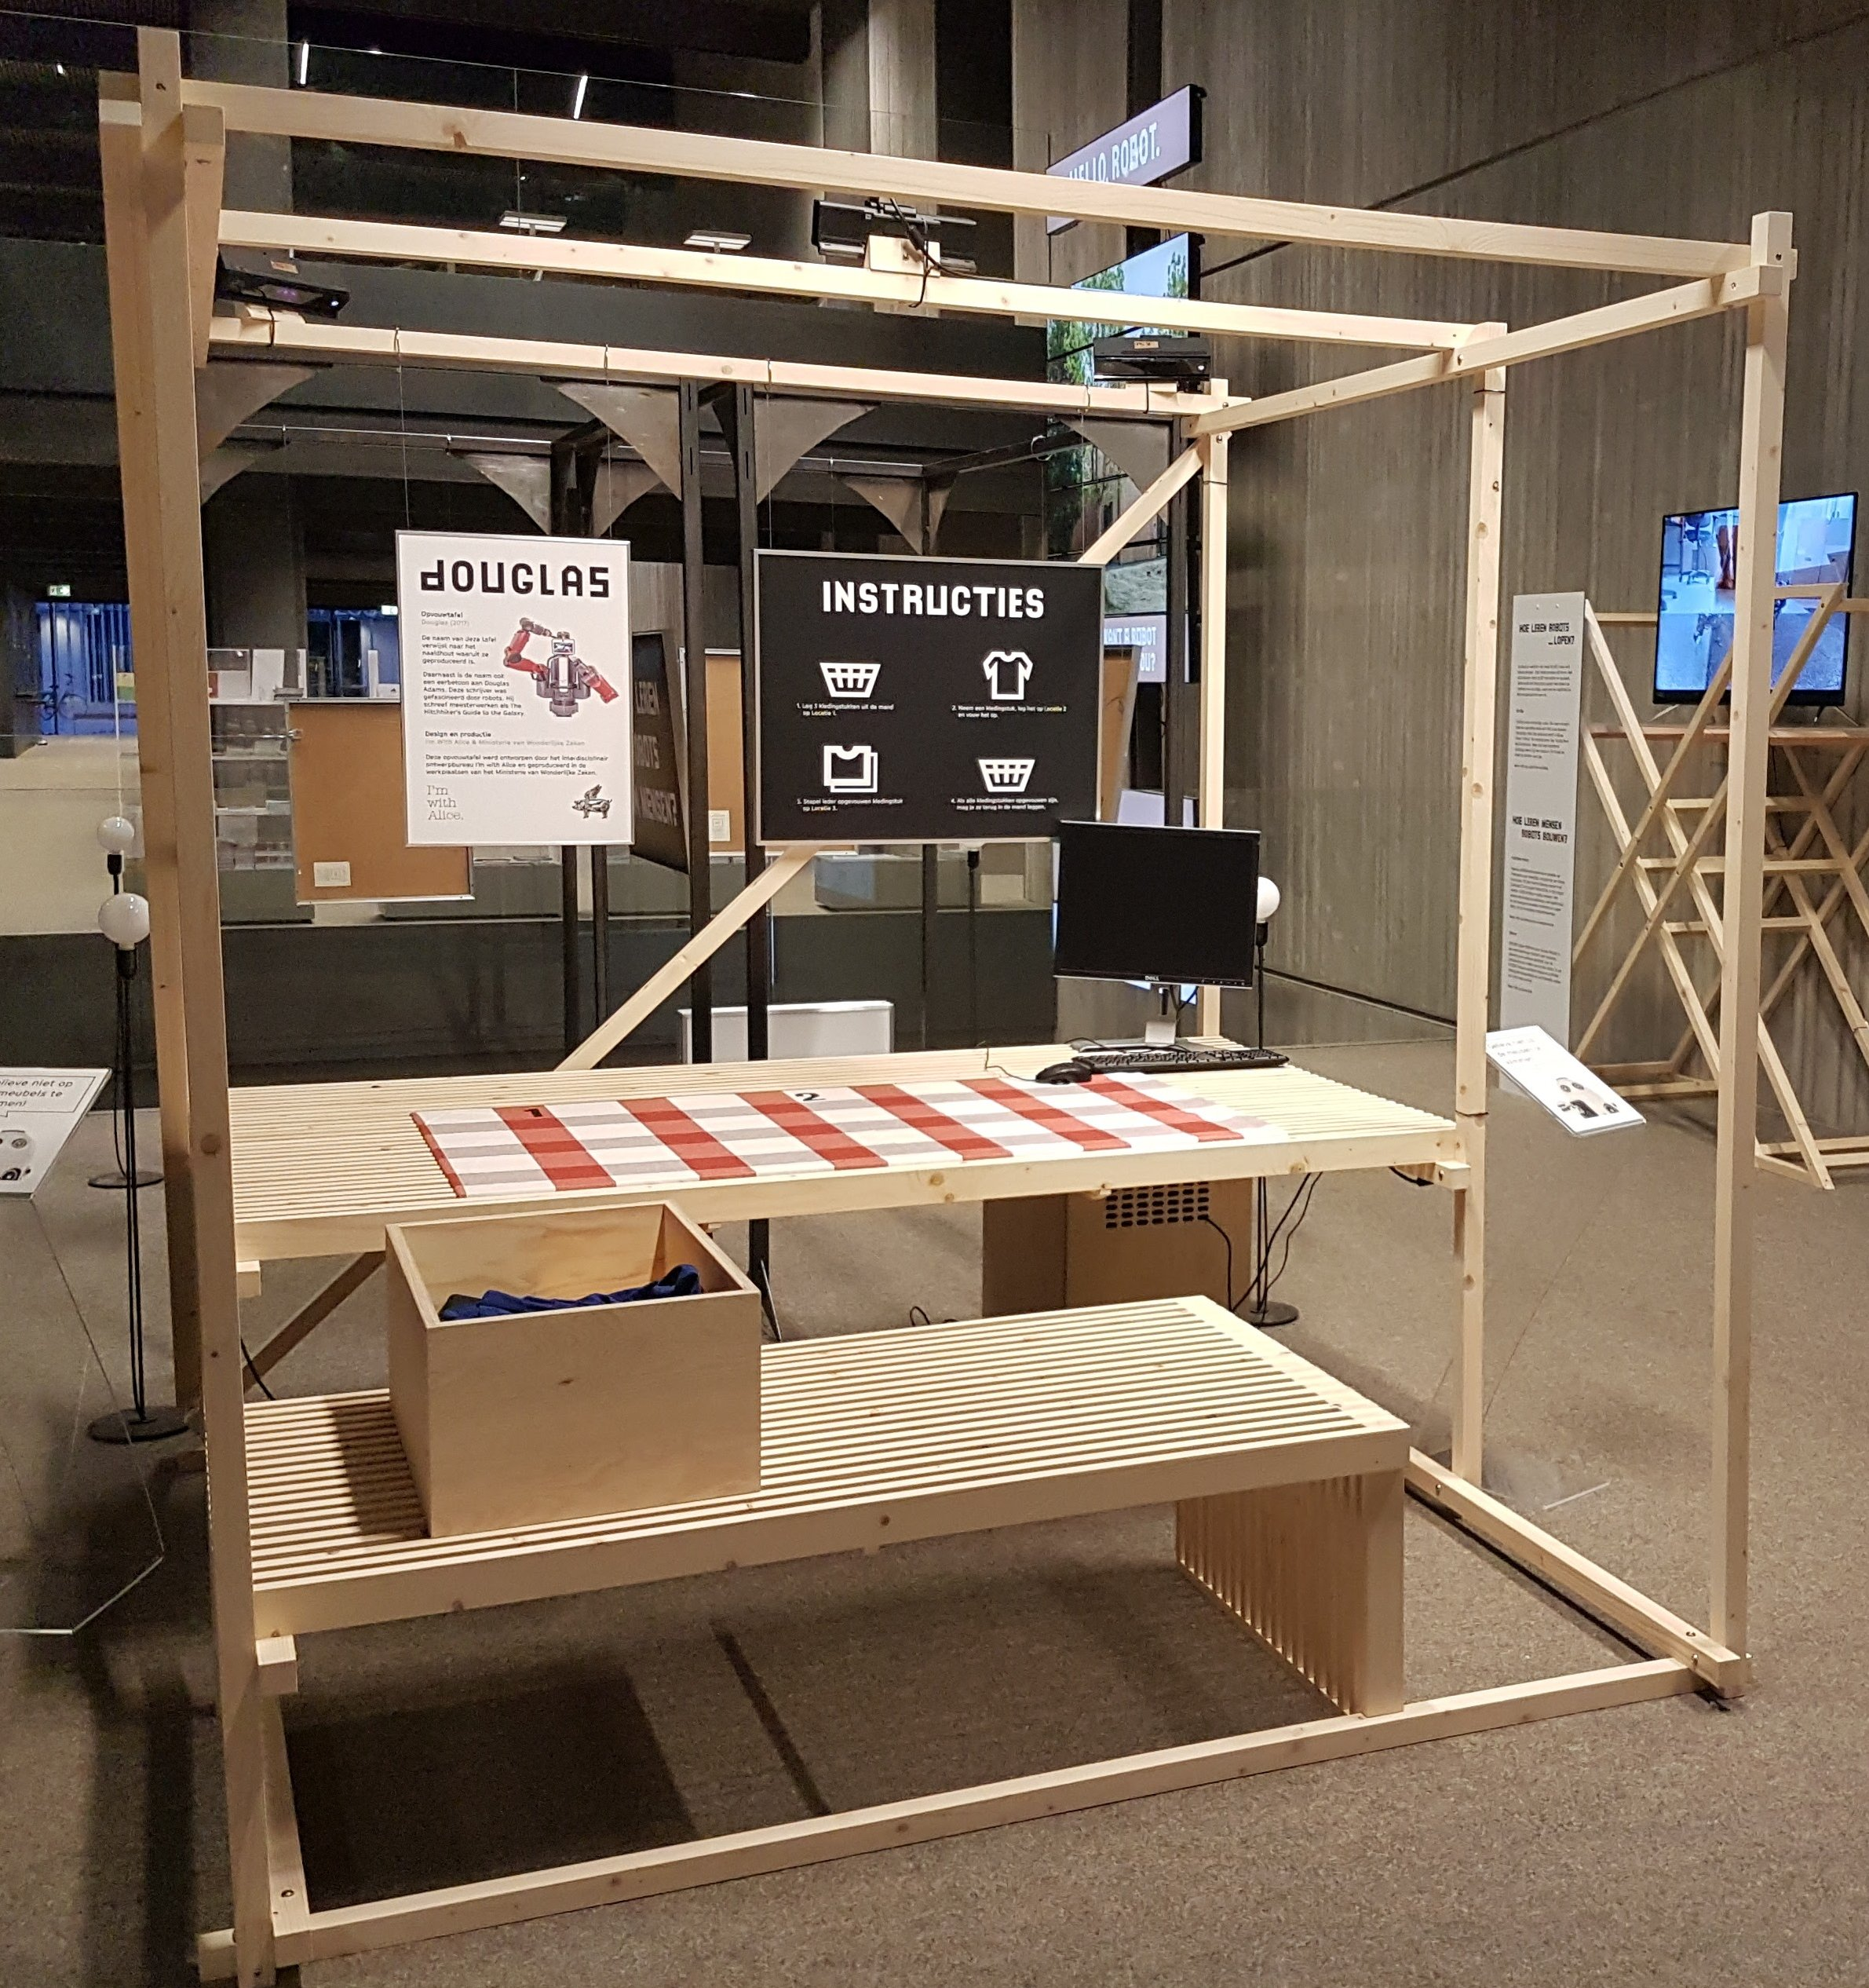
\includegraphics[width=0.45\textwidth,keepaspectratio]{figures/douglas_empty} 
    \caption{Picture of our folding table setup to crowdsource video demonstrations in a public library. } % There are three Kinect cameras mounted on top of the table that capture the human folding demonstrations. %We provide easy and clear instruction to introduce consistency in the demonstrations. 
    \label{fig:douglas}
  \end{figure}
  
  % Onze oplossing 
  To fill the gap in learning the robotic folding task from human demonstrations, we provide a dataset that aims to accelerate research by providing crowdsourced video demonstrations of people folding clothing. Kinect cameras mounted on a folding table recorded the task executions from multiple perspectives. This resulted in $1000$ folding demonstrations in the wild. We segmented and labelled the data such that a subtask of each demonstration can be queried. We provide anonymized RGB images and depth values from three fixed perspectives, together with the skeleton keypoint trajectories. We are confident our dataset of video demonstrations of people folding clothing will accelerate research for learning of the robotic folding task and can be used for action recognition tasks on multiple temporal levels, for example detecting different folding methods and detecting the steps associated with folding textile.
  
  \begin{figure}[h]{}
       \centering
       \begin{subfigure}[b]{0.32\textwidth}
           \centering
           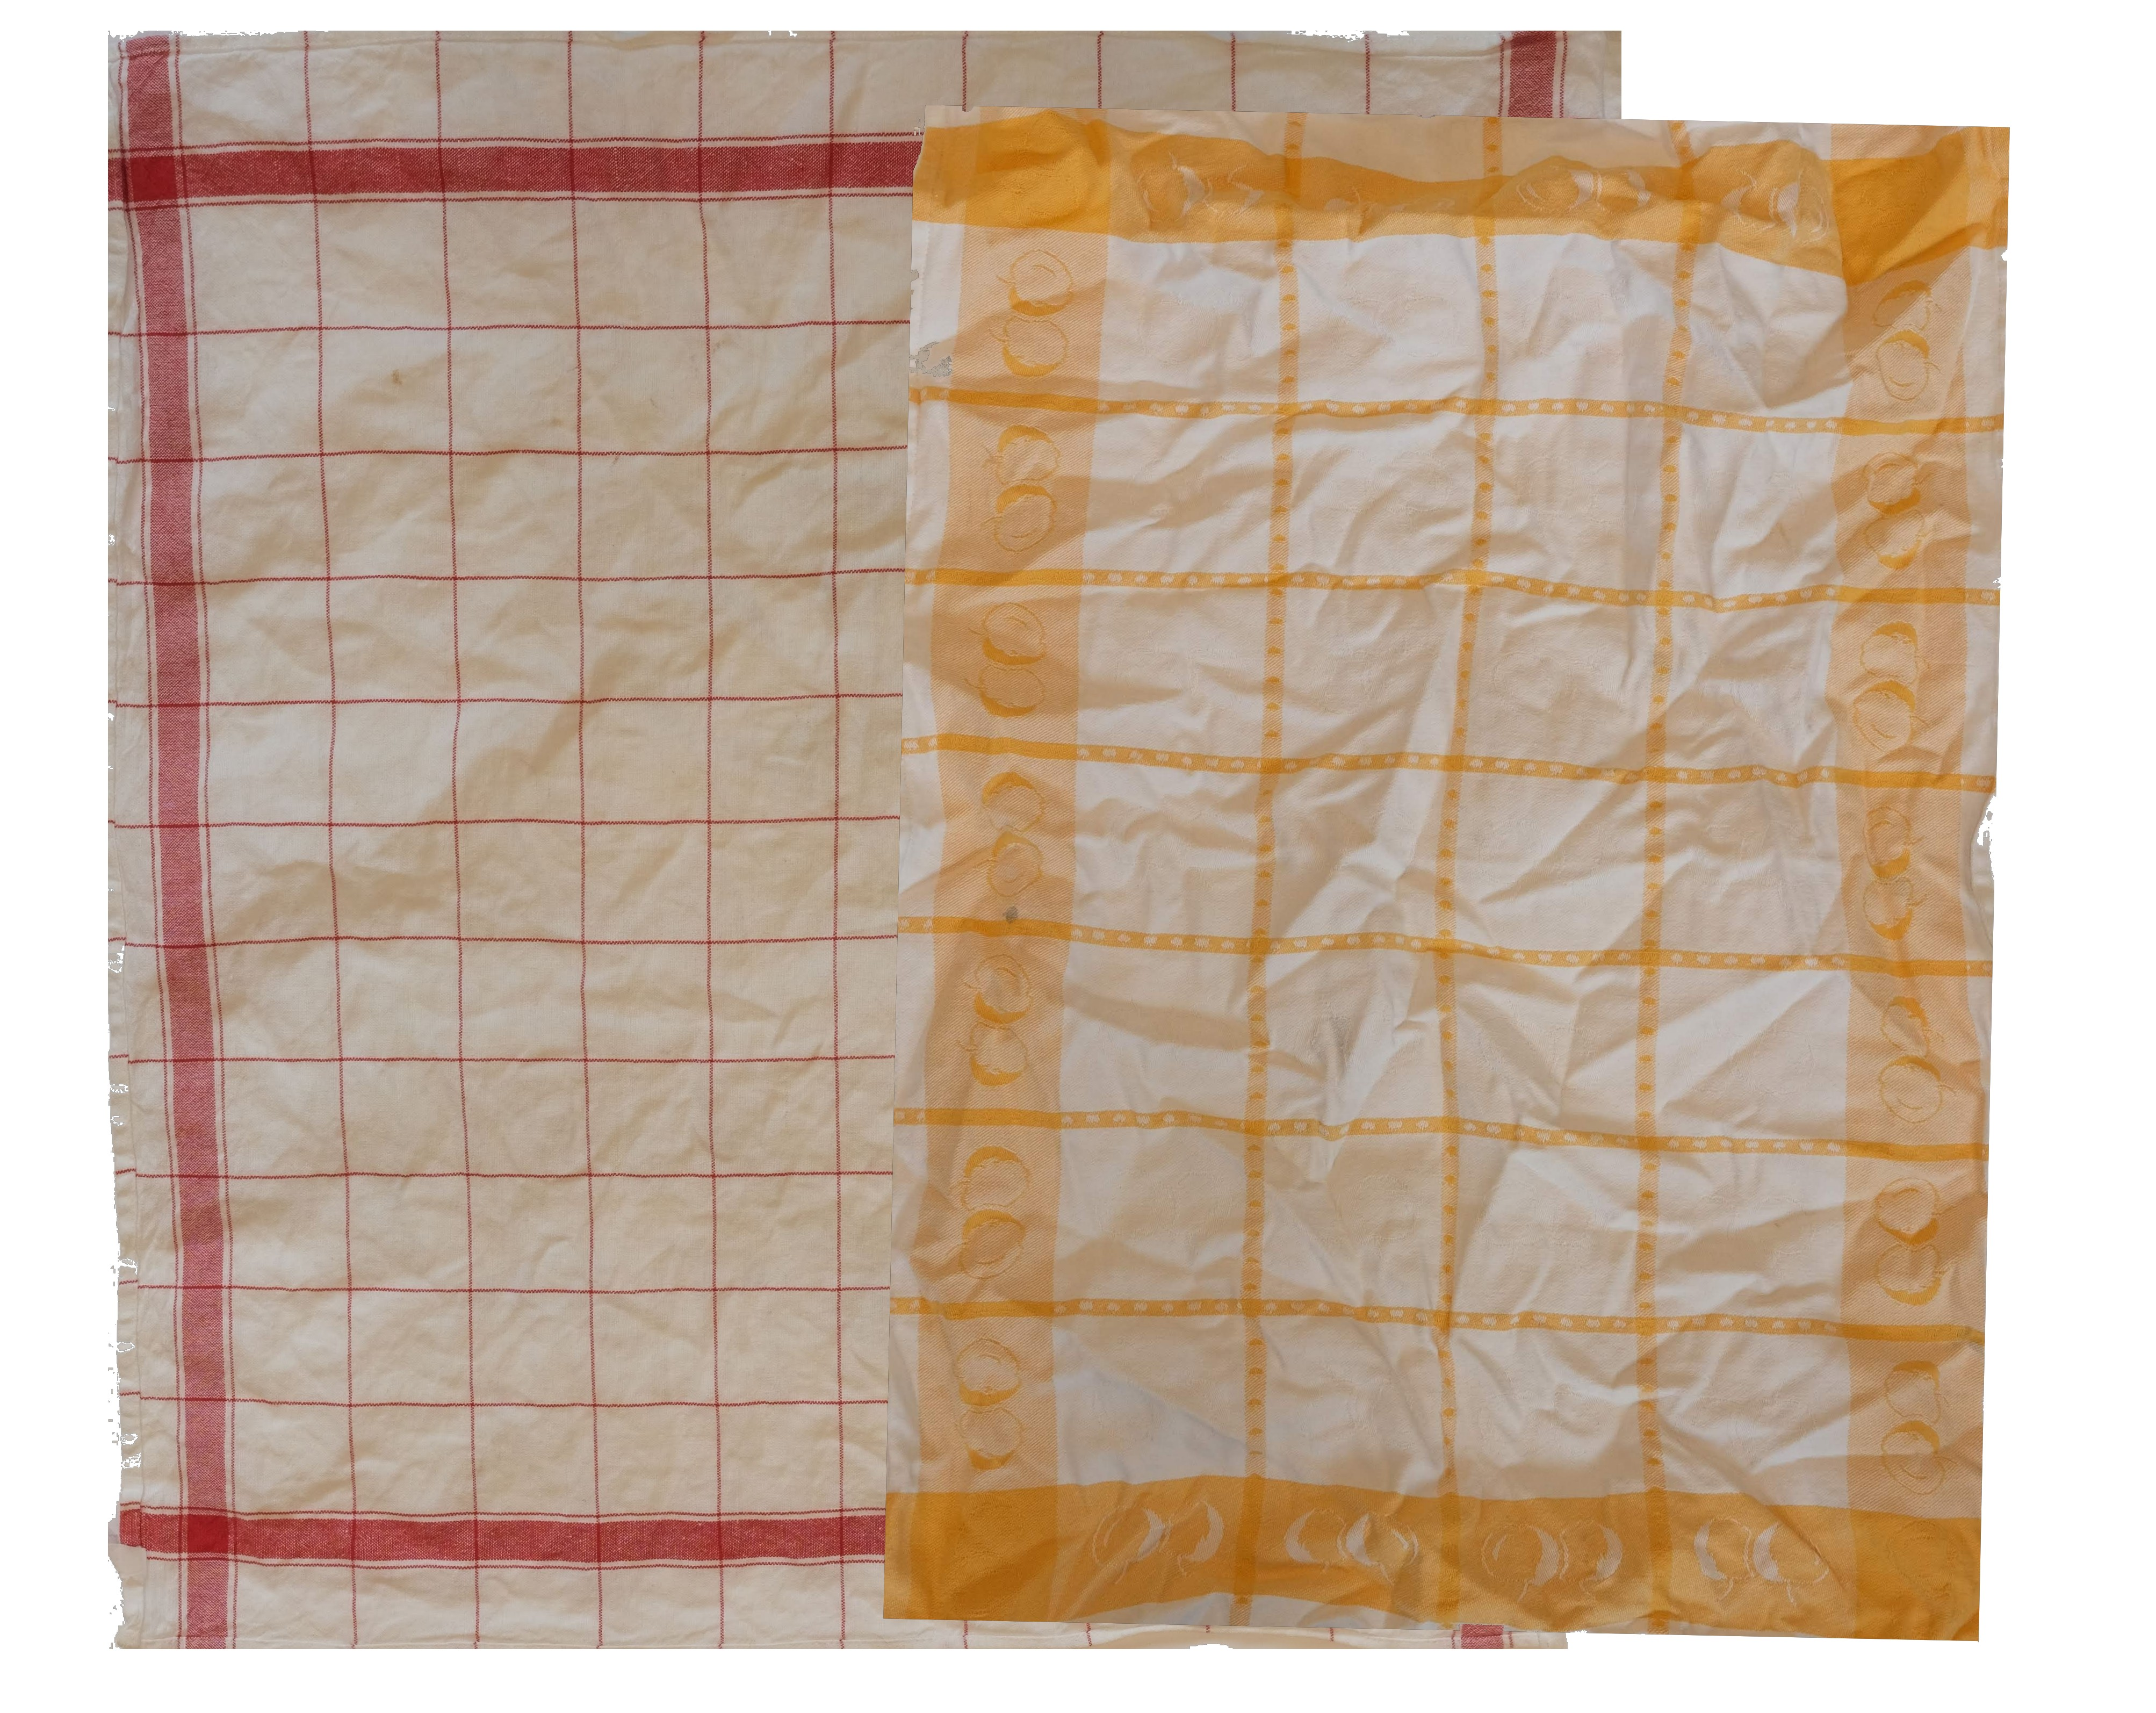
\includegraphics[width=\textwidth]{figures/towels.jpg}
           \caption{The towels in the dataset contain different textures and are of similar size.}
           \label{fig:towel}
       \end{subfigure}
       %\hfill
       \begin{subfigure}[b]{0.32\textwidth}
           \centering
           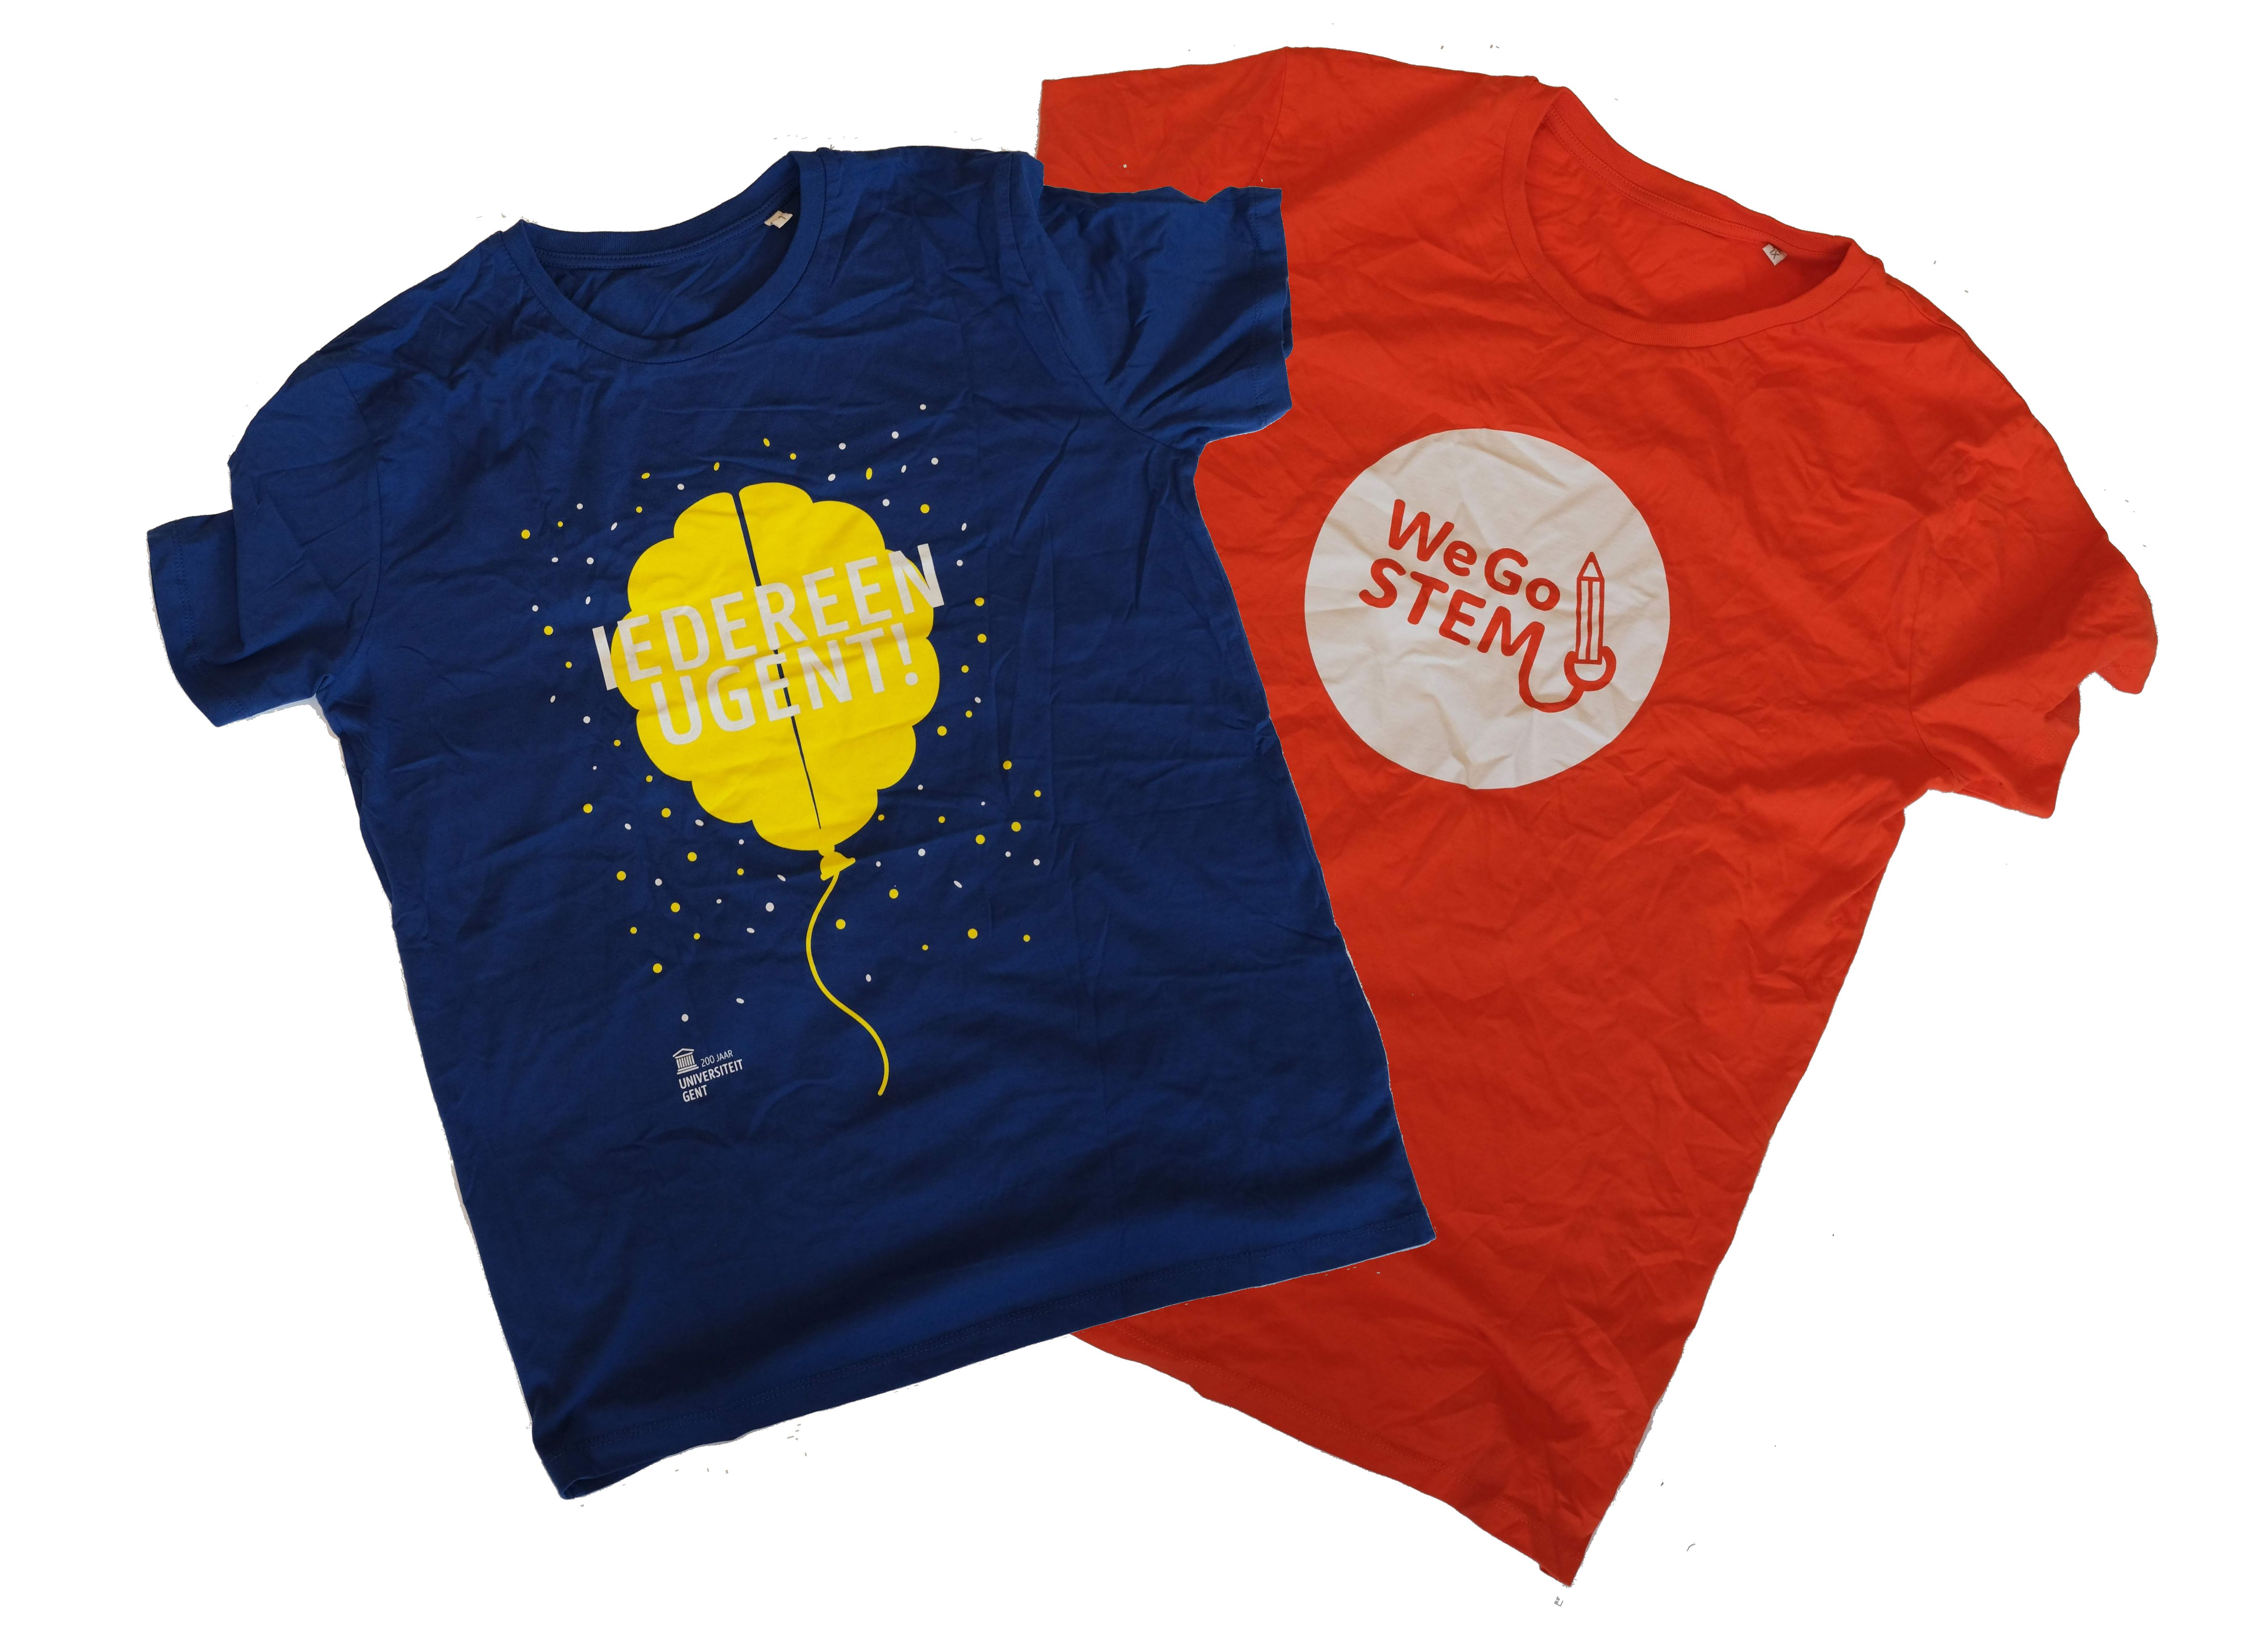
\includegraphics[width=\textwidth]{figures/shirts.jpg}
           \caption{The sizes of the t-shirts range from small to extra large and consists of a multitude of colours.}
           \label{fig:shirt}
       \end{subfigure}
       %\hfill
       \begin{subfigure}[b]{0.32\textwidth}
           \centering
           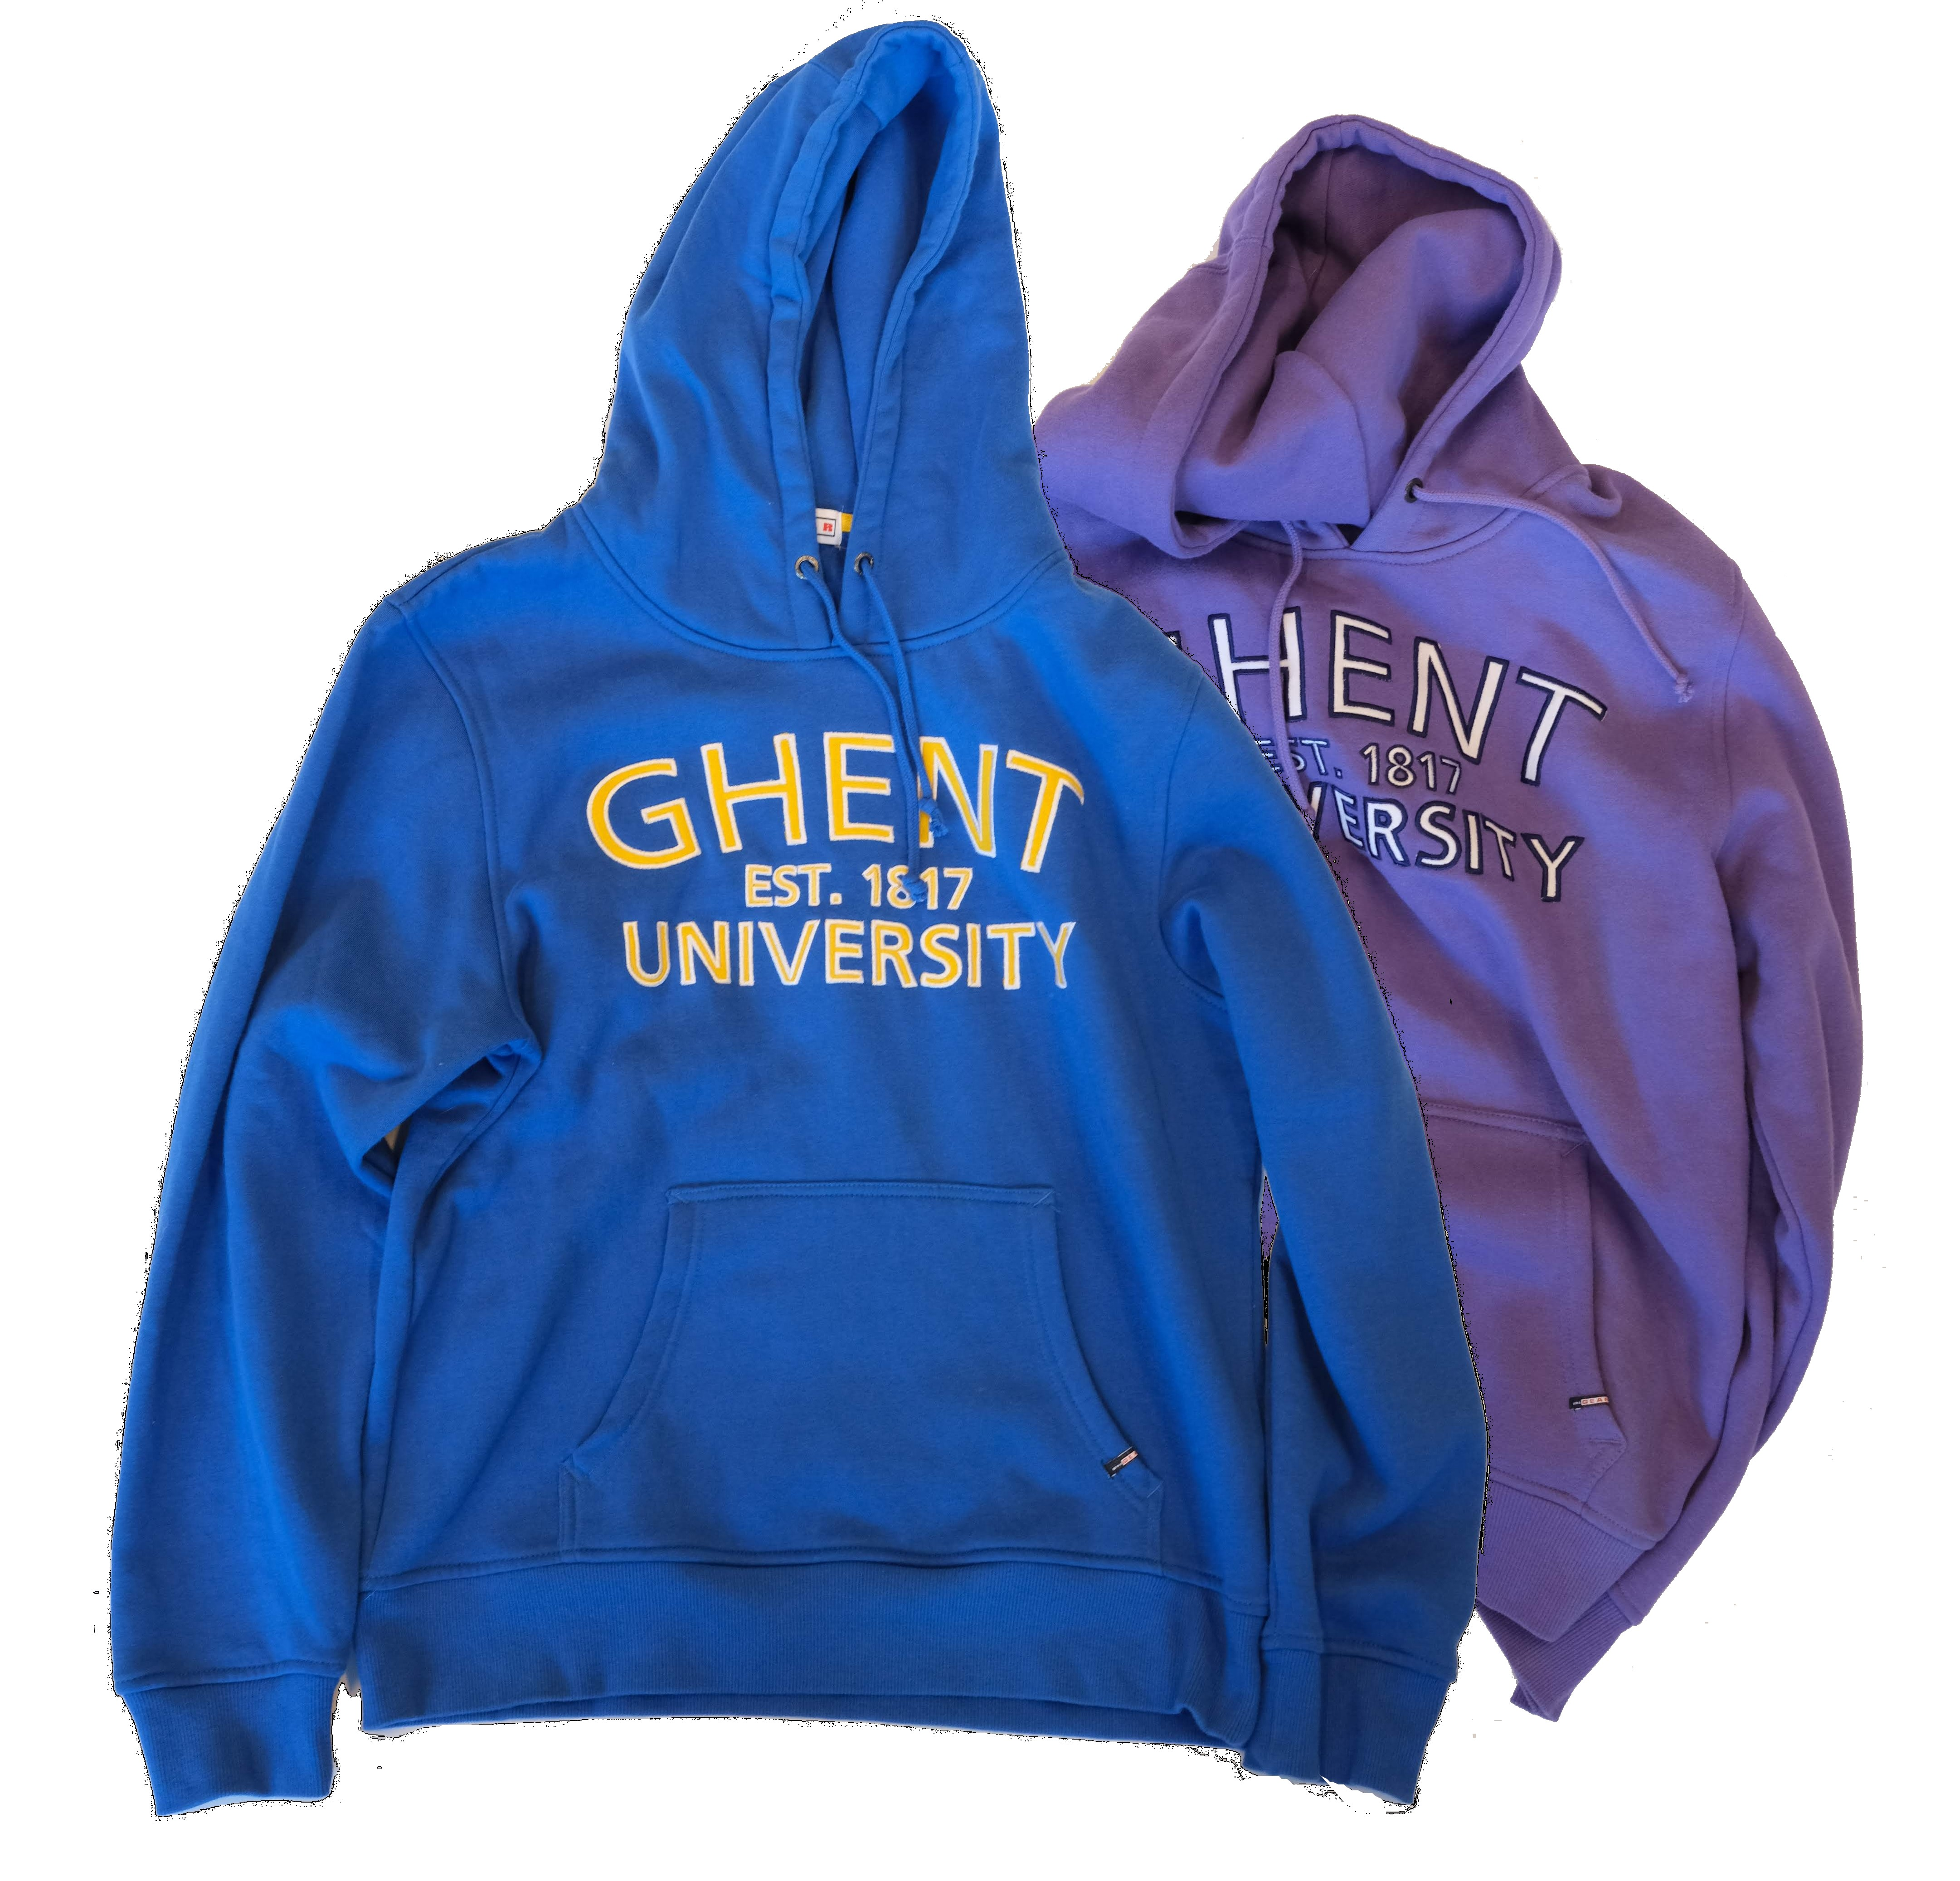
\includegraphics[width=\textwidth]{figures/hoodies.jpg}
           \caption{The hoodies are arguably the hardest piece of textile to fold in the set. There are two hoodies with a different colour.}
           \label{fig:hoodie}
       \end{subfigure}
          \caption{ The set of textiles that has to be folded by the participants consists of hoodies, t-shirts and towels with a variety of sizes, colours and textures. }
          \label{fig:textiles}
  \end{figure}
  
\section{Crowd-sourcing folding demonstrations}
\todo{Volgende stuk herverdelen en aandikken in volgende subsecties}
%Doel: beschrijven van de setting, waarom een citizen science project, hoe georganiseerd en ingericht. 

% Citizen science project motivatie 

We gathered a heterogeneous dataset of folding demonstrations using a community-based participatory approach \autocite{English2018}. We involve citizens by requesting them to demonstrate their method to fold clothing on a folding table with cameras. Using posters, an instructional video and warning symbols around the folding table setup, we made it explicit that participants will be recorded on video on video for the purpose of research in the domain of robotics and AI. We collected no demographics or other kind of personal information. This setup allows us to capture different folding strategies and manipulation varieties within a folding method. The participants consist of a combination of students and visitors of a public library in the third largest city in Belgium. This avoids selection bias in the dataset. Furthermore, we place our setup within a small exhibition on research in robotics to inform the public about learning strategies for robots and give an answer to an innate fear in society that self-learning robots could lead to a loss in jobs \autocite{Fleming2019}. \par

% Beschrijving tafel
To capture video task demonstrations, a special-purpose folding table was designed and constructed which can be seen in Figure~\ref{fig:douglas}. The table is a beam-like, wooden skeleton structure consisting of a tabletop, a bench, camera mounting points, a basket, and a locker. The participant is required to fold the clothing on the working surface. The tabletop is detachable in order to apply different tablecloths as a means to introduce additional variety in the dataset. As we require the demonstrator to sit while performing the task, we place a large bench attached to the wooden frame. The bench also obstructs observers to prevent occlusion and distraction during task execution. There are three Kinect v2 cameras mounted on top of the table. They capture the perspective from the task executor and two top corner video streams to deal with occlusion. They are placed approximately $160$ cm and $183$ cm from the center of the folding table in order to capture the complete folding sequence demonstration. The Kinect cameras provide RGB and depth information at a resolution of respectively $1920$x$1080$ and $512$x$424$ pixels. The wooden basket is attached to the bench and serves as a proxy for a laundry basket. Finally, a locker safeguards the workstation embedded in the table. We use the libfreenect2 driver \autocite{Xiang2016} to capture the frames and process the six video streams, RGB and depth information, online using an AMD Ryzen 1700X CPU. Because of the high bandwidth requirements of the Kinect cameras, we limit the frame rate to $10$ FPS. \par 

\begin{figure*}[th] % TODO make sure this figure appears after the textile pictures and before the folder structure 
  \centering
  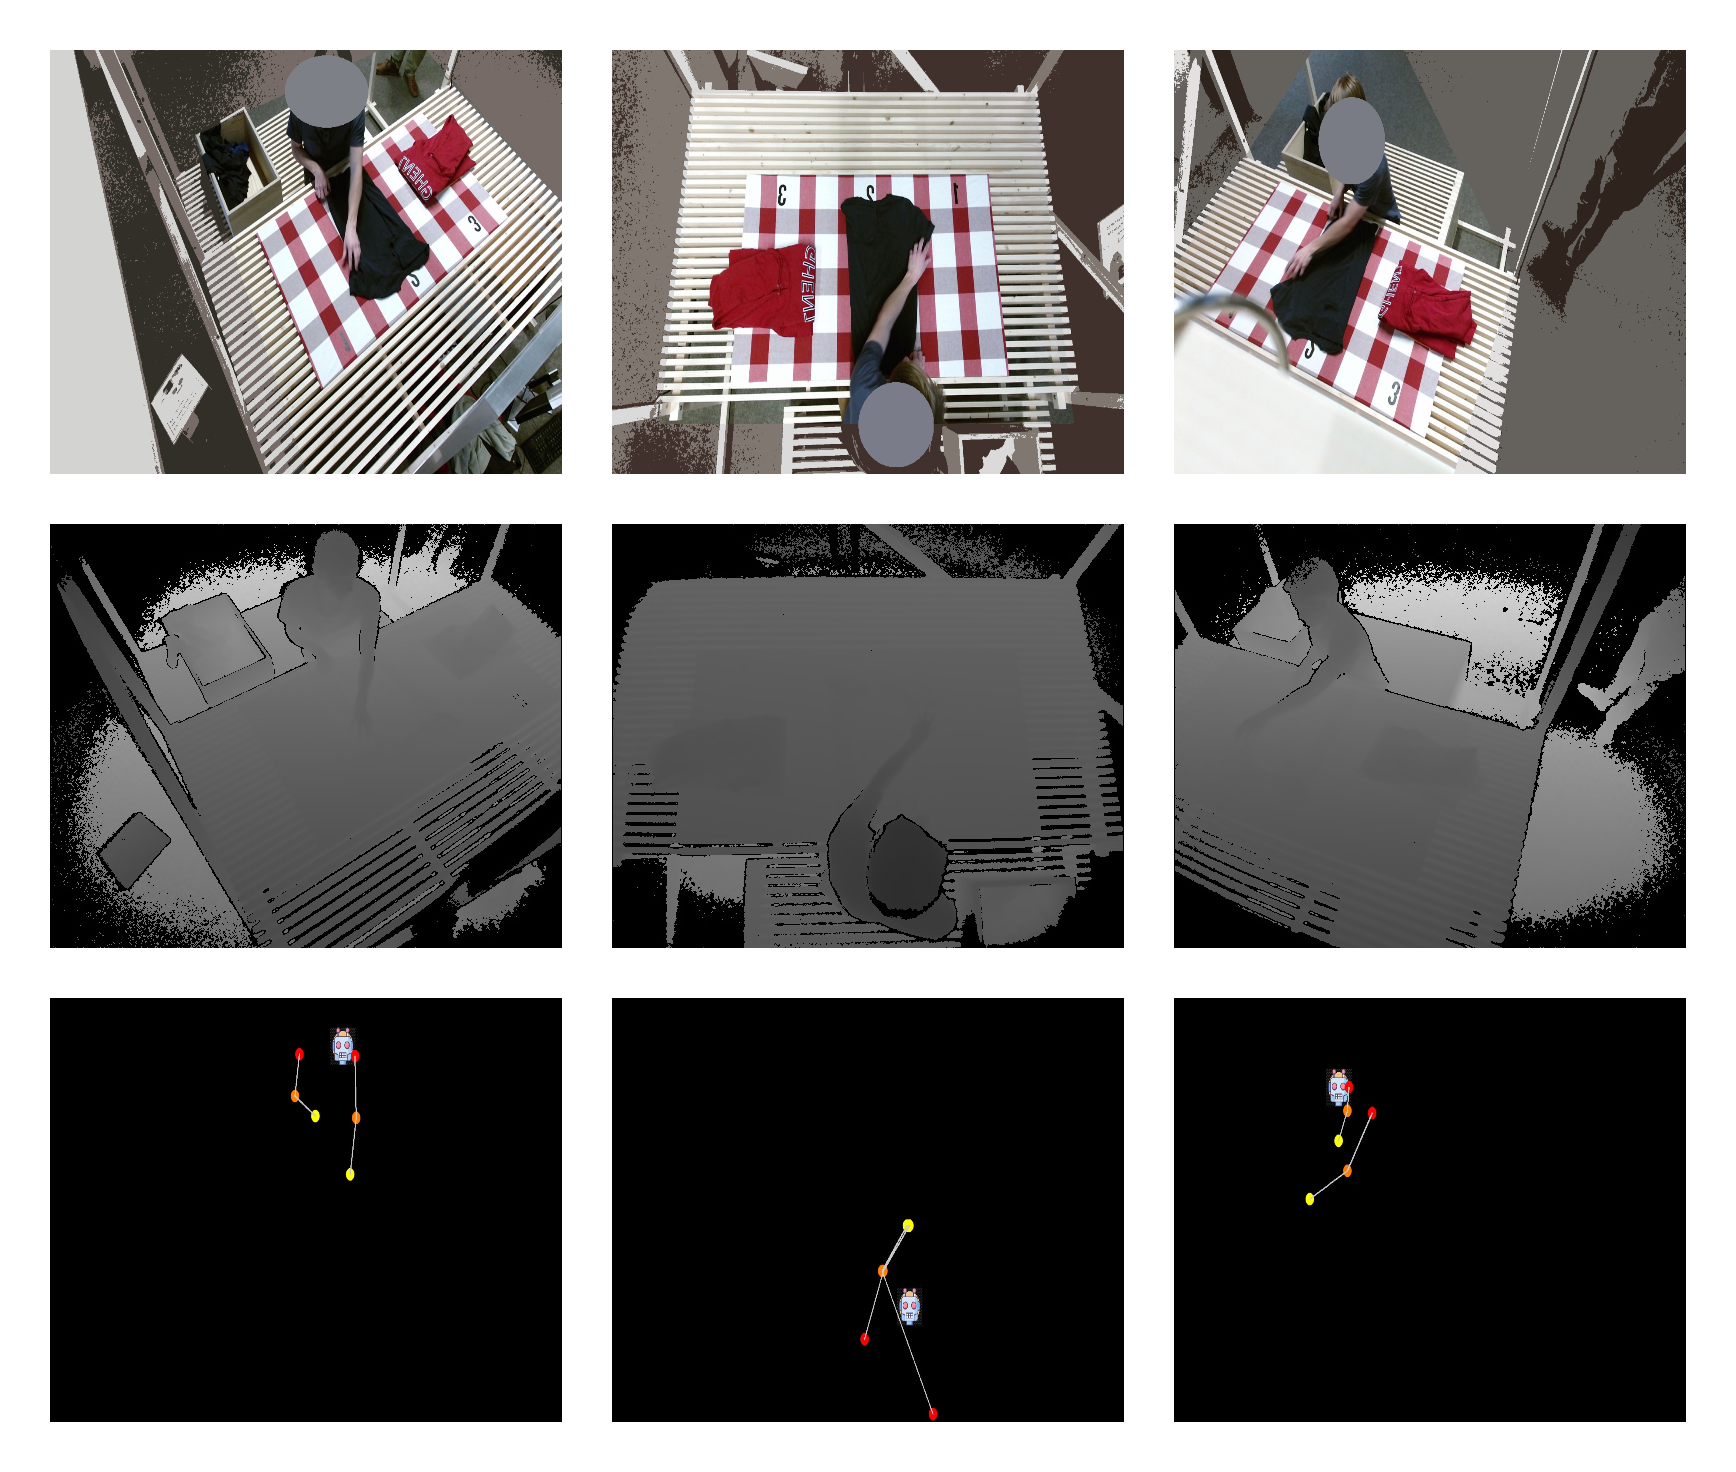
\includegraphics[width=\textwidth,keepaspectratio]{figures/3x3-sample} % height=1.0\textheight
  \caption{ \textbf{Example output from our dataset.} We provide RGB images, depth registrations and skeleton keypoint trajectories of $6.5$ hours of human demonstrations of folding clothing. The RGB images are anonymized without compromising image fidelity or disturbing the folding demonstration. The videos are segmented such that one sample represents the folding of one piece of textile.}
  \label{fig:fig1}
\end{figure*}

% Aanpak --> instructies
To structure the participants' task demonstrations, we provided a four-step instruction list: (1) place randomly selected clothing out of the basket on the left side of the table, (2) fold one textile at the time in the middle of the table, (3) collect it at the right of the table and (4) put all textile back in the basket. We made an instructional video and put up a poster containing these instructions to avoid high variance in task execution.  \par 

% Activity detection
Because the folding table is stationed in a public space with mostly no human supervision, we leave it recording throughout the project. To avoid running out of storage and filtering frames without human activity, we run an activity detection heuristic based on changes in the pixel values of the video stream. To guarantee ample observations, we also actively visited the setup to attract and inform visitors about the project. We noticed our presence had a positive effect on the number of visitors willing to participate in the data crowdsourcing project. \par 

% Welke stukken textiel zitten er in? 
The included types of textiles in the basket are towels, t-shirts, and hoodies. Examples are shown in Figure~\ref{fig:textiles}. We excluded trousers as they are hard to flatten from a sitting position. Socks were also excluded from the set because folding socks require high-dexterous, fine manipulation actions that would not be visible from the mounting position of the cameras.  \par

After capturing the example demonstrations, we cleaned all false positive recordings from the database, sliced the recordings into single-piece folding demonstrations and manually labelled subtasks. The subtasks consist of grasping isolated clothing, unfolding, flattening, folding and stacking it on top of each other. We defined exact definitions of these subtasks in Table~\ref{table:subtask_def} in order to consistently label the video fragments. As data quality plays an important role for learning algorithms, we annotated the data ourselves to ensure there is consistency in the labelling between samples. These subtask labels can, for example, be used in reinforcement learning for reward engineering or hierarchical learning and for the training of action recognition systems. Skeleton keypoints were extracted from all frames in post-processing using AlphaPose \autocite{Fang2017}.

\begin{table}[]
\small\centering

\begin{tabular}{|p{2.3cm}|p{5.5cm}|}
\toprule
Subtask & Definition \\
\midrule 
Isolated grasping & The subject selects grasping points to remove a piece of textile from a heap of multiple textile pieces and isolates the selected textile. \\
Unfolding & The subject selects grasping points and executes manipulation trajectories in order to remove a fold. \\
Flattening & The subject executes manipulations in order to remove wrinkles from a piece of textile which can be in any state. \\
Folding & The subject selects grasping points and executes manipulation trajectories in order to bring the textile into a folded configuration. \\
Stacking & The subject grasps the textile and moves it outside the folding area, possibly stacking it on top of a pile of folded textiles. \\
\bottomrule
\end{tabular}
\caption{Definitions used to label the subtasks in the folding task}
\label{table:subtask_def}
\end{table}


\section{Technical setup}
\subsection{Folding table {\tiny hardware}}
\subsection{Robust real-time recording {\tiny recording software, detection system, fault tolerance}}
\subsection{Post processing {\tiny clean-up, labeling etc}}
\section{Folding demonstrations dataset}
% RESULTATEN

The observations in the datasets are captured over the course of two months at two different public locations. The set contains $1000$ folding demonstrations of three different types of textiles. This amounts up to $8.5$ hours of folding recorded in $304820$ frames. We registered four different types of folding methods. We segmented each video into chunks of single folding demonstrations and provide RGB frames, depth information, annotations, pose trajectories and timestamps of the different steps in the folding task. The content and how to access and use our dataset is described in the remainder of this section.  

% ---------------------- Folder structure -------------------------
\subsection{Folder structure}
The dataset is segmented into folding demonstrations of a single piece of textile. This structure is visible in the folder hierarchy in Figure~\ref{fig:folder_structure}. For each example demonstration, we find annotations and timestamps indicating the subset of the task. Because we have three cameras mounted on fixed positions on the folding table, we put the colour, depth and pose registrations in the folders \textit{left}, \textit{middle} and \textit{right} which represent the viewpoint in front of the table. 

\begin{figure}[htb]
  \centering
  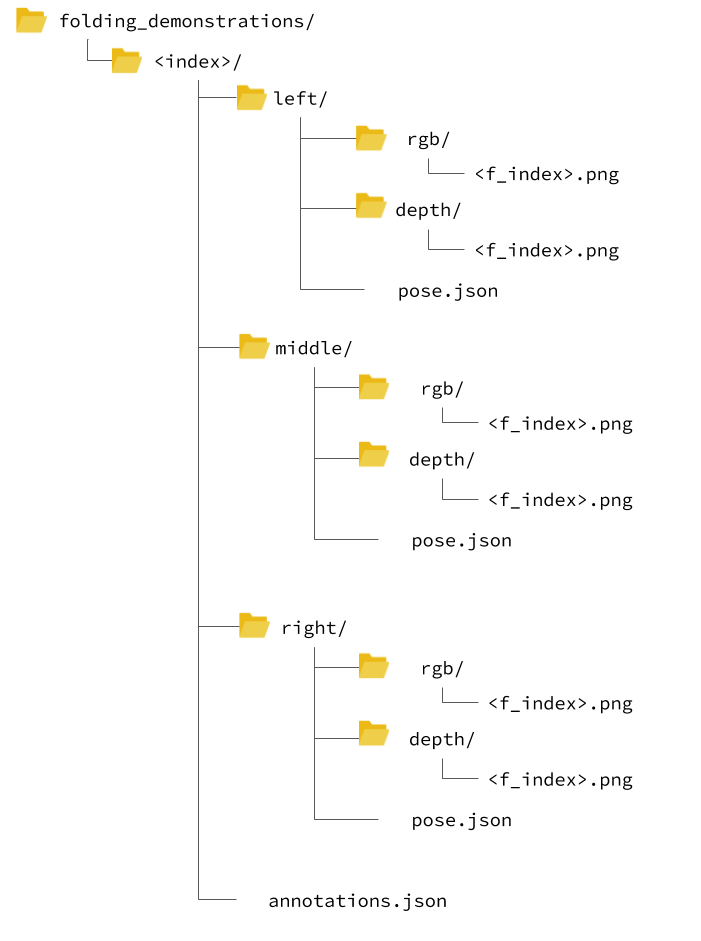
\includegraphics[width=0.45\textwidth,keepaspectratio]{figures/folder_structure_with_icons.png} 
  \caption{ \textbf{Folder structure of the folding demonstration dataset.} There is a folder per folding demonstration, indicated with \textit{<index>}. Each sample contains labelled data in the annotations json file. The images are grouped per perspective and contain rgb and depth images. There are also joint positions available per video perspective. }
  \label{fig:folder_structure}
\end{figure}


% ---------------------- DATA FORMAT -------------------------
\subsection{Data format}
The RGB images captured with the Kinect cameras are compressed with the \textit{x265} codec. We use the intrinsic camera calibration parameters to modify the images according to the depth correction. All RGB frames are anonymized by applying colour quantization to the corners of the frame and pasting an ellipsoid colour patch around the face of the demonstrator which was tracked using AlphaPose \autocite{Fang2017}. \par

Each sample in the dataset contains annotations in the \textit{annotations.json} file. The labelled information and data format can be seen in Listing~\ref{lst:annotations}. We label which type of textile is being folded and which folding method is being used. We distinguish four categories of folding methods, labelled from \textit{a} to \textit{d}. These categories represent an increasing amount of complexity to learn a certain folding strategy. For example, folding method \textit{a} extensively uses the table to make folds. In contrast, method \textit{b} represents demonstrators making vertical folds while lifting the cloth in the air. Method \textit{c} categorizes folding strategies which requires crossing the hands. Finally, method \textit{d} captures all different strategies not described by the former folding categories, for example rolling up the cloth. All four folding strategies can be used on all types of cloth in the dataset. The different types of textile are labelled as \textit{hoodie}, \textit{shirt} or \textit{towel}. The distribution of the folded clothing is as follows: $88\%$ of the folded clothing are shirts, $9\%$ are towels and $3\%$ hoodies. The timestamp is in \texttt{YYYY-MM-DD HH:MM:SS} format. Given that the data is crowdsourced, some variation exist in the way participants followed the high-level process instructions. For example, some demonstrators fold the clothing immediately out of the basket instead of first collecting the pieces on the left side of the table. To indicate to which extent the given process instructions are being followed, we included a quality label in the annotations. This label is useful if consistent, high-quality samples need to be sampled. In the dataset, $86\%$ follow the given instructions, $12\%$ make one deviation while $2\%$ do not follow the given high-level instructions. The exact definitions of the quality label are shown in Table~\ref{table:quality_def}.

\begin{table}
\begin{tabular}{|p{3.2cm}|p{4.6cm}|}
\toprule
Quality label & Definition \\
\midrule 
Follows instructions & The instructions were followed exactly. \\
Slight variation on instructions & One deviation was made from the instructions. \\
Very different from instructions & Two or more deviations were made from the instructions. \\
\bottomrule
\end{tabular}
\caption{Because not all demonstrators follow the given high-level task instructions, we define a quality label of which the definitions are given in this table.}
\label{table:quality_def}
\end{table}

\begin{lstlisting}[language=json, caption=annotations.json description, label={lst:annotations}, float,floatplacement=H, captionpos=b]
{
    "id": 0,
    "timestamp": "2018-09-30 19:35:06",
    "cloth_type": "hoodie",
    "location_id": 0,
    "nb_frames": 579,
    "folding_method": "a",
    "demonstration_id": 0,
    "nb_folds": {
        "0": 0,
        "66": 1,
        "94": 2,
        "118": 3
    },
    "subtask_changes": {
        "0": "isolated_grasping",
        "42": "unfolding",
        "112": "folding",
        "300": "stacking"
    },
    "quality": "follows instructions"
}
\end{lstlisting}

We labelled each part of the video with a descriptor indicating which step in the folding process the demonstrator is going through. The different steps are named \textit{isolated\textunderscore grasping}, \textit{unfolding}, \textit{flattening}, \textit{folding} and \textit{stacking}. 

We provide human skeleton keypoint trajectories in the file \textit{pose.json}. There are pose trajectories available for each camera perspective per folding sample. The joint positions are stored in the JSON format visible in Listing~\ref{lst:pose}. There is a score associated with each pair of $x$ and $y$ coordinates. This variable, ranging from $0$ to $1$ indicates the detection confidence that a certain joint is at the given location. In general, the coordinates for every joint positioned beneath the shoulders are less reliable because the subject is sitting on a bench with the legs occluded by the table. We consider this not a problem because the coordinates of the joints of the two arms are reliable and are of importance for the folding task. 


\begin{lstlisting}[language=json, caption=pose.json description, label={lst:pose}, captionpos=b]
{
    frame_nr: {
        "LElbow": [x, y, score],
        "RElbow": [x, y, score],
        "LShoulder": [x, y, score],
        "RShoulder": [x, y, score],
        "LWrist": [x, y, score],
        "RWrist": [x, y, score],
        ... 
        "confidence": 100.0
    }
}
\end{lstlisting}


% ---------------------- WEBSITE   -------------------------

\subsection{Project website and helper scripts}
Along with the data, we provide helper scripts in Python which are available at \url{https://github.com/adverley/folding-demonstrations}. The data can be loaded by calling \mintinline{python}{FoldingDemonstrationDataSet(home_dir)}. We expose the data as a nested dictionary, embedded in a list. This enables an intuitive interface for accessing the data by iterating over the \mintinline{python}{FoldingDemonstrationDataSet} object and querying specific fields with corresponding key in square brackets. For example, \mintinline{python}{data[0].annotations['clothing_type']} queries the type of clothing being folded in demonstration $0$ while \mintinline{python}{dataset[42][0]['rgb']['left']} returns the first RGB image of video demonstration $42$. A more complete and general-purpose example can be found in Listing~\ref{lst:python_example}.

\begin{listing}[htb]
\caption{Example code how to query the dataset}
\label{lst:python_example}
\begin{minted}[breaklines,breakanywhere, 
mathescape,
 numbersep=5pt,
 frame=single,
 numbersep=5pt,
 xleftmargin=0pt,]{python}
 
from folding_demonstrations.dataset import FoldingDemonstrationDataSet

# Set to the directory where the folding demonstrations dataset is stored
home_dir = '/media/data/folding_data_output'

# Load the data
dataset = FoldingDemonstrationDataSet(home_dir)

# Iterate over data and query available information
for sample in dataset:
    random_frame_nr = 42
    frame = sample[random_frame_nr]
    rgb_left = frame['left']['rgb']
    rgb_middle = frame['middle']['rgb']
    rgb_right = frame['right']['rgb']
    depth_l = frame['left']['depth']
    depth_m = frame['middle']['depth']
    depth_r = frame['right']['depth']
    subtask = frame['subtask']
    reward = frame['reward']
    pose = frame['pose']

\end{minted}
\end{listing}


\section{Conclusion}

In this paper, we introduce a video dataset with human demonstrations of folding textile, captured via a citizen crowdsourcing project. With this dataset, we aim to fill in a gap in learning deformable objects manipulation, bootstrapped by human examples. We provide $1000$ demonstrations with RGB images, depth frames, and joint pose trajectories captured from three perspectives simultaneously. We labelled the data with subtask annotations, folding method, and textile type. Our goal is to provide robotics researchers with a real-world dataset to accelerate the learning from human demonstrations for deformable object manipulation.

\end{document}